\documentclass[letterpaper,12pt]{article}
\usepackage{biblatex}
\addbibresource{sources.bib}
\usepackage{graphicx}
\usepackage{hyperref}
\usepackage{cleveref}
\usepackage{tabularx}
\crefname{section}{Sec.}{Secs.}
\Crefname{section}{Section}{Sections}
\Crefname{table}{Table}{Tables}
\crefname{table}{Tab.}{Tabs.}
\usepackage{amsfonts}
\graphicspath{ {./images/} }

\begin{document}

\title{Improving Transparency and Mitigating Hallucinations in LLMs: A Survey}
\author{Sydney Newmark}

\maketitle

\section{Abstract}
Large language models (LLMs) have impressive performance in parsing language and generating natural-sounding responses. However, LLMs have several problems related to the accuracy of those responses. They may ``hallucinate" (provide incorrect or irrelevant information), provide confidently incorrect responses and explanations, and may not sufficiently explain their reasoning. This paper explores existing solutions to these problems, such as Chain-of-Thought prompting to improve explainability, calculations to measure uncertainty in responses (called ``semantic uncertainty"), and Mixed-contrastive Learning to reduce the generation of hallucinations. We then combine several of these solutions in a proposal which modifies the structure of the GPT-series of models in an attempt to simultaneously reduce hallucinations, use uncertainty in choosing LLM responses, and increase explainability.

\section{Introduction}

Generative artificial intelligence for text has been rapidly growing in popularity during late 2022 and the early half of 2023, with ChatGPT receiving one million users in just five days \cite{statistachatgpt}. Other widely available models have also entered the space, with Microsoft's Bing Chat, based on GPT-4, launching, as well as Google Bard, which uses the PaLM 2 model. Large language models have been widely praised for their ability to automate some tedious writing tasks. Additionally, large language models have been implemented in integrated development environments to provide LLM-assisted code completion through Microsoft's GitHub Copilot, and for general queries typically reserved for a traditional search engine, like Google.

Much of the work in natural language generation (e.g., GPT) has been focused on producing models capable of generating realistic-sounding text, with less emphasis put on whether a model's responses are factually correct. This proves to be a problem when users attempt to substitute a large language model, like ChatGPT, for a traditional search engine. With no way to verify that a model's responses are accurate, they must resort to verifying the results through other means, most likely through a traditional search engine they were attempting to substitute. Tied to factual accuracy are hallucinations, where a model assumes a piece of context that was not explicitly provided to it by the user or says things that are factually incorrect. In writing tasks, this may result in subtle incorrect information being included, which the user may not review before using the model's output.

This paper reviews existing methods for improving LLM accuracy, conveying uncertainty, and mitigating hallucinations. Drawing on our findings in the literature, we then propose a set of modifications to the structure of the GPT-series of models using CoT prompting, MixCL, and Mixture-of-Experts, which may improve these qualities.

\section{Related Work}
Artificial intelligence has been defined as the intelligence of machines, which can have many different sub-fields, including computer vision (self-driving cars), search engines (Google), and generative or creative tools (ChatGPT, Stable Diffusion). The latter category has been of particular note since OpenAI's release of ChatGPT as a public research preview on November 30, 2022. ChatGPT is a large language model (LLM) whose primary purpose is to engage in conversations with human users based on the questions or requests users provide to the model.

Prior to the advent of transformers, natural language processing tasks widely employed a mechanism known as recurrent neural networks (RNNs). An RNN is a method of processing input tokens (groupings of approximately one word each) that suffers from notable drawbacks in the context of large language models. RNNs process tokens sequentially, creating a state vector (a sequence of tokens) containing the $n^{th}$ preceding tokens along with the current token, $n$. Consequently, they suffer from something known as the vanishing gradient problem, which describes the lack of precise information about preceding tokens by the time processing of input has finished. This can inhibit or completely prevent further training. The other notable drawback of RNNs is that they are difficult to parallelize because of their sequential nature. Parallelizability is a valuable property for improving performance in neural networks, because an individual layer of the network can be computed simultaneously. Transformers, on which modern LLMs such as ChatGPT are based, provided an alternative framework for approaching the processing of input sequences based on what is known as the \textbf{attention mechanism}. This allows parallel processing of input sequences by linking an input token with other related input tokens to capture structure and context that would have been lost with a RNN approach.

As of July 2023, OpenAI and Google are the two primary companies with accessible, consumer-facing chat programs based on transformer-backed large language models. ChatGPT uses OpenAI's GPT-3.5-turbo and GPT-4 models, while Google's Bard uses the PaLM 2 model. LaMDA (Language Model for Dialogue Applications), also produced by Google, is a conversational AI model trained on dialogue and published in 2021. OpenAI's GPT models use a method called Reinforcement Learning with Human Feedback (RLHF) to train, by which humans determine which kind of output texts are ``good" based on their interpretation of specific criteria. This is subsequently input back into the unsupervised learning process, guiding the model to produce more text similar to that which humans have declared good outputs. GPT-4 is also trained using RLHF, the main difference between it and both GPT-3.5-turbo and Google's two large language models being the use of a Mixture-of-Experts (MoE) approach \cite{gpt4moe}. GPT-4 has eight expert models, each slightly larger in parameter count than GPT-3.5-turbo, with each specialized for a certain type of task. MoE works by taking the input text, giving it to each of GPT-4's expert models, and then employing a gating model to choose the best answer produced by any of the experts \cite{shazeer2017outrageously}. The best answer will then be provided to the user.

\section{Explainability}

Although LLMs are capable of creating natural-sounding text, how well an LLM can explain itself (``explainability") is vital to providing users with more useful responses. Explainability measures the depth and specificity of text produced by a LLM to explain how it arrived at an answer. As an example of this measure, consider the statements in \cref{fig:CoT}. The output in \textbf{Standard Prompting} receives a lower explainability score based on its lack of supplemental text for the answer provided, while \textbf{Chain-of-Thought Prompting} receives a higher score because it provides factually accurate supplemental text to support the answer provided. Explainability is a crucial element of LLM output because it allows a user to understand an LLM's reasoning. This is particularly of note when the only alternative is a black box where a user is forced to either fact check the LLM or blindly trust its response.

\begin{figure}[htbp]
    \caption{An example provided by Wei et. al. showing outputs with varying degrees of explainability \cite{wei2022chain}}
    \label{fig:CoT}
    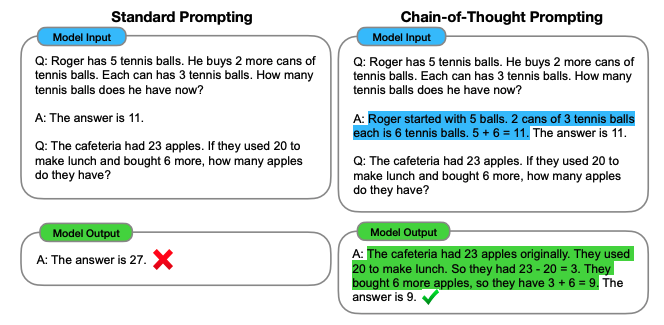
\includegraphics[width=12cm]{chain-of-thought}
    \centering
\end{figure}

\subsection{Chain-of-Thought Prompting}
\label{sec:cot}
A method called Chain-of-Thought (CoT) prompting is a prompt engineering technique that uses the model input to provide examples of the reasoning that should be expected in outputs \cite{wei2022chain}. As shown in \cref{fig:CoT}, CoT reasoning is the process by which an answer can be obtained; a thought process. In the CoT output example, instead of only providing a single numerical answer, the model produced additional details, such as intermediate steps.

This technique has had empirical gains in complex reasoning on tasks including arithmetic, commonsense, and symbolic reasoning. This is a task that had previously been unable to be achieved through merely scaling the model size. While in-context few-shot learning via prompting has had success in question-answer (QA) tasks, limitations arise when reasoning abilities are required, and this cannot be trivially solved by increasing model size. Fundamentally, CoT relies on a prompt split into three parts: input, chain of thought, and output. By providing demonstrations of this process, large language models can generate chains of thought. This approach led to improved solve rates, i.e. accuracy, in arithmetic reasoning, common sense reasoning, and symbolic reasoning tasks. The approach was tested on PaLM, LaMDA, and GPT models. In the GSM8K benchmark, the strongest performing model, PaLM, at 540B parameters, surpassed a solve score of 50\% using CoT prompting, while only reaching 20\% without CoT prompting. Improvements for all three models were comparable or negative at smaller parameter counts, but improved upon non-CoT prompting for the PaLM, LaMDA, and GPT models at larger parameter counts.

\subsection{Scientific Debugging: AutoSD}

Scientific Debugging is a method of debugging by which developers maintain an iterative debugging log of five steps:

\begin{enumerate}
    \item Hypothesis, where a description is given of what the bug could be;
    \item Prediction, of an expected outcome if the hypothesis is true;
    \item Experiment, to verify the prediction;
    \item Observation, the result of an experiment; and
    \item Conclusion, a judgement of the hypothesis.
\end{enumerate}

Kang et al. focused on the importance of explanation of automated program repair results in scientific debugging \cite{scidebug}, including techniques such as Fault Localization (FL), of which 85\% of developers agree that providing rationale is important. The study presented describes one method of prompt engineering. The process consists of providing a definition of Scientific Debugging (SD), complemented with examples of hypotheses, predictions, experiments, observations, and conclusions. After an initial prompt is prepared, the process, called AutoSD, generates a hypothesis on what is wrong with the code and how it can be fixed. It then produces and executes code to validate that hypothesis, after which the process will terminate and either generate a fix or loop from the beginning. AutoSD was evaluated on the Almost-Right Human Eval (ARHE) dataset, which was created by taking human solutions to bugs and modifying them such that exactly one test fails, creating ``almost" right code. When comparing AutoSD to prompting an LLM for a fix without any specific prompt engineering techniques (LLM-Base), it performed ten points better than LLM-Base on plausibly correct and correct bug fixes. In the Defects4J 1.2 benchmark, AutoSD performed 11 points worse than LLM-Base, while in the Defects4J 2.0 benchmark, AutoSD performed 3 points better than LLM-Base.

\subsection{Discussion}

These approaches for higher quality explanations demonstrate how providing specific context to a large language model in input text can have a substantive impact on explainability by providing a ``template" for the LLM to follow when producing its output. The CoT approach implements this by including within the prompt examples of expected reasoning. Similarly, AutoSD describes the process of SD and examples of hypotheses along with other key aspects of SD. Both CoT and AutoSD are methods which ``train" the LLM to simulate or imitate procedures which lend themselves to explainable outputs.

\section{Uncertainty}
Related to the problem of explainability in large language models is the problem of reliably measuring \emph{uncertainty}. This is important because without an accurate measure, it is not worthwhile to use generated outputs as a reliable source of information \cite{kuhn2023semantic}. Large language models have been shown to produce confidently incorrect answers to questions commonly asked of them. This often requires the user of an LLM to validate the answer it provides, partially or entirely undermining the value of using the program to start with. Below, we describe some major approaches for uncertainty estimation in large language models.

\subsection{Semantic Uncertainty}
\label{sec:semantic-uncertainty}

Kuhn et al. estimated what they call semantic likelihoods, which are probabilities attached to the meanings of text. They used semantic likelihoods to compute semantic entropy, a measure of uncertainty across those different meanings \cite{kuhn2023semantic}. Practically, entropy, and by extension, semantic entropy, is a measure of the likelihood of certain text being true.

Consider the question ``What is the first element of the Periodic Table?" and three answers to the question: ``The element is Hydrogen", ``Hydrogen", and ``Oxygen." Assigning an arbitrary probability to each corresponding to the likelihood it is true, we may obtain 0.5, 0.4, and 0.1, respectively:
\begin{itemize}
    \item ``The element is Hydrogen": 0.5
    \item ``Hydrogen": 0.4
    \item ``Oxygen": 0.1
\end{itemize}
Computing the \emph{semantic} likelihood simply requires adding statements which \emph{mean} the same thing, since they should be considered equivalent. Following this procedure, we group ``The element is Hydrogen" and ``Hydrogen" together, and add their probabilities, yielding 0.9 as the semantic likelihood that the first two answers are true, and a 0.1 semantic likelihood that ``Oxygen" is true:
\begin{itemize}
    \item ``The element is Hydrogen" + ``Hydrogen": 0.9
    \item ``Oxygen": 0.1
\end{itemize}
Grouping the likelihoods in this manner results in a much lower semantic entropy than standard entropy (calculated from the original ``standard" likelihoods), where a lower entropy is interpreted as less \textbf{uncertainty} in the output.

The algorithm to estimate semantic uncertainty consists of first generating a set of answers from a model according to a particular probabilistic distribution. Then, the answers are clustered by \textbf{semantic equivalence}, which results in sets of answers which share the same meaning with respect to the context of the question being asked. The semantic equivalence is calculated using a novel algorithm based on bi-directional entailment. The algorithm returns that two sentences are \textbf{equivalent} if one sentence entails the other sentence and vice versa. For example, consider the question, ``What is the capital of Paris?", and two sentences in response: ``The capital of Paris is France," and ``Paris is the capital of France." Each of the two sentences necessarily imply that the other sentence is true, so they are semantically equivalent. Finally, the semantic entropy is calculated. The semantic entropy measure was evaluated using the area under the receiver operator characteristic curve (AUROC), which yields values closer to 1 when the probability that a randomly chosen correct answer has a higher uncertainty score  than a randomly chosen incorrect answer. Semantic entropy predicted model accuracy better than normalized entropy, entropy, and lexical similarity on TriviaQA, a question-answer dataset, and CoQA a conversational question-answer dataset. In TriviaQA, at the highest parameter count of the model, semantic uncertainty reached an AUROC score of approximately .83, while normalized entropy, the second-highest score, was approximately .78. In CoQA, at the highest parameter count of the model, semantic uncertainty reached an AUROC score of approximately .77 and normalized entropy reached a score of approximately .74.

Duan et al. responds to the notable limitation Kuhn et al. did not address: that some tokens are more relevant to semantic meaning of a text than other tokens, yet are treated equally when estimating uncertainty, termed ``generative inequalities" \cite{duan2023shifting}. They introduce the idea of Shifting Attention to Relevance (SAR) uncertainty estimation. For example, consider the phrase, ``density of an object," as a response to the question, ``What is the ratio of the mass of an object to its volume?" With the previous method proposed by Kuhn et al., the token ``of", while not very relevant to the response, contributed the most uncertainty. SAR uncertainty estimation shifts ``attention" to the most relevant components (i.e. ``density" in the above example) of a response.

To estimate SAR uncertainty, attention shifting is performed on both the token level and at the sentence level. For each token, a relevance score is calculated, which is used to emphasize or de-emphasize token entropy based on those relevance scores. At the sentence level, sentences which have a high generative probability, i.e., a more compelling sentence, are emphasized. Evaluations of this method show that SAR improves on the Semantic Entropy calculations proposed by Kuhn et al. on both CoQA and TriviaQA using OpenAI's state-of-the-art GPT models.

\subsection{Discussion}

A training process could employ a strategy, like the computation of semantic entropy, as a feedback mechanism of the mode to minimize incorrect generations and generations unlikely to be correct beyond some threshold. Calculation of semantic entropy on specific components of a model's output could also be used as part of the generation process to highlight areas, either text-based within the model itself, or as part of a client user interface, where the uncertainty estimation determines the model is likely not correct in an assertion.

\section{Mitigating Hallucinations}
\subsection{Hallucinations}
An undesirable behavior in some use cases for large language models, such as code generation, is its tendency to ``hallucinate," where it infers context, either correct or incorrect, about a situation while presenting it as if it were fact. In code generation, this may manifest as function names or libraries present in code samples which do not exist. Alternatively, consider the question, ``How many deaths has the virus caused in the United States?" If a model's training data consists of many instances of virus referring to COVID-19, it may ``hallucinate" that the user asked about that particular virus. If that was indeed what the user was asking about, the ``hallucination" may have been beneficial.

Nick McKenna et al. designed an experiment to test two causes of hallucinations in large language models, \textbf{The Veracity Prior} and \textbf{The Relative Frequency Heuristic}  \cite{mckenna2023sources}. The Veracity Prior is a measure of whether a statement is consistent with the LLM training data. Consider a premise, ``More than 19 million people live in the New York City metropolitan area," and a hypothesis, ``New York City is the most populous metropolitan area in the United States." The experiment uses the Levy/Holt dataset, which contains premise-hypothesis pairs of the form ``Given [some premise], is it true that [some hypothesis]?" The premises and hypotheses were inserted into a prompt template that was fed to the model. If a premise \textbf{entails} a hypothesis, then if the premise is true, it necessarily follows that the hypothesis is also true. The results of an experiment to determine the reliance on the \emph{veracity prior} using LLaMa, GPT-3.5, and PaLM, showed an approximately 2x higher chance of predicting that a premise entails a hypothesis when the hypothesis has been previously judged to be truthful. Using prior knowledge, i.e. memorization of hypotheses in training data, may result in hallucinations in situations where knowledge is provided to an LLM as context by the user, and the LLM then uses information not present in the user-provided context when providing an answer.

The Relative Frequency Heuristic assigns a label of \textbf{Entail} if a premise, such as ``More than 19 million people live in the New York City metropolitan area" is found less frequently in the dataset than a hypothesis, such as ``New York City is the most populous metropolitan area in the United States." This is relevant because specific terms in text corpora are normally less frequently present (\textbf{corpus-frequency}), while the opposite is true for general terms. Thus, less corpus-frequent terms may entail more corpus-frequent seen terms. The heuristic is measured according to Google N-grams, which charts the frequency of search strings in Google's text corpora. This is used as an approximation of the natural distribution of text. Results of an additional experiment showed that when Natural Language Inference (NLI) test samples, such as the premise-hypothesis pairs found in the Levi/Holt dataset, conform to the relative frequency heuristic, despite the existence of no semantic relationship between the premise and hypothesis, models are more likely to falsely report \textbf{Entail}. False positive rates, i.e. frequency at which models reported a semantic relationship between a premise and a hypothesis, were measured at 1.5x, 1.7x, and 2.0x for LLaMA, GPT-3.5, and PaLM, respectively.

\subsection{Mixed-contrastive Learning}
\label{sec:mixcl}
Weiwei Sun et al. proposed a method called Mixed-contrastive Learning (MixCL) to mitigate hallucinations by large language models \cite{mixcl}, by \textit{contrasting} the ground truth with samples of ``confusing" knowledge, where ``confusing" knowledge is knowledge that has a substantial likelihood of causing the model to hallucinate. This approach reduces the probability of generating answers incongruent with the ground truth. MixCL consists of two primary steps: \textit{negative sampling} and \textit{mixed-contrastive learning}. The first step uses ``positive knowledge" ($z^+$; factual and relevant) and a sampling of ``negative knowledge" ($z^-$; not factual or not relevant). While existing contrastive learning strategies are able to reduce hallucinations at the sentence level, MixCL seeks to mitigate hallucinations at the \textit{span} level, i.e. a non-overlapping subset, or sequence of tokens, within a sentence. It achieves this through a process of extracting spans from both positive and negative knowledge, mixing positive and negative knowledge spans together to form new sequences, and optimizing the model using \textit{mixed-contrast loss}, a loss function based on contrastive learning. For example, consider two knowledge statements about former Apple CEO Steve Jobs: ``He was born and raised in San Francisco" (positive knowledge) and ``He was born and raised in Cupertino" (negative knowledge). Mixing these spans together involves taking one span from a snippet of $z^+$, like ``Paris," and substituting it for the corresponding span from a snippet in $z^-$, like ``Cupertino". The results of an experiment on the Wizard of Wikipedia dataset show that MixCL achieves higher scores with human evaluations than all the language-model-based methods under realistic conditions for informativeness, relevance, factuality, and humanlikeness. Weiwei Sun et. al. used the Fleiss' kappa statistical measure to determine reliability of agreement between the human evaluations on MixCL. They measured a score of over 0.60, indicating substantial agreement.

\subsection{Discussion}
The tendency of large language models to hallucinate based on the level of understanding it has of a situation's context can lead to incorrect assumptions based on a hypothesis being true when given an unrelated premise (\textbf{Veracity Prior}). In addition, the frequency of a hypothesis in the text corpora can influence a model's judgement of whether a premise entails that hypothesis (\textbf{Relative Frequency Heuristic}. MixCL reduces hallucinations of irrelevant and incorrect spans.

Mitigating hallucinations may be an important step towards more accurate uncertainty measures of large language model outputs as it reduces the probability of measuring a large uncertainty value for any given output. Furthermore, since hallucinations are a fundamental problem of the current design of large language models, limiting hallucinations can enable more precise fine-tuning of truthfulness using semantic uncertainty measures of output in model training and inference.

\section{Proposed Method}
\label{sec:proposed-method}

We propose a framework which aims to improve three primary qualities in the current state-of-the-art large language models: explainability; uncertainty; and hallucinations. Hallucinations are the primary focus area to improve as it decreases the value of explained responses and uncertainty calculations. If an explanation contains many span-level hallucinations which make an argument incorrect in subtle ways, that explanation is minimally valuable for the user.

Training LLMs to produce more robustly explained answers to questions is also crucial in the pursuit of reflecting confidence levels, because uncertainty can be measured more precisely. While standalone numerical or text outputs can be measured for uncertainty \cite{kuhn2023semantic}, such an uncertainty measurement provides no useful information to an end user, who may be interested in specific parts of a response which may not be correct. Uncertainty estimation of parts of an explanation could be used to produce text by which the LLM informs the user where it is uncertain. However, this requires that the model be trained to reflect a level of uncertainty in its explanations.

Using the GPT-3.5 model structure as a base, we propose that a mixed-contrastive learning (\cref{sec:mixcl}) framework be integrated into the model training cycle. During the unsupervised learning component of the cycle, the model will take into account minimization of the mixed-contrastive loss function when calculating adjustments to parameters. In the supervised reinforcement learning component, human reviewers will sample responses from the model and extract positive ($z^+$) and negative ($z^-$) knowledge spans to be used by the mix-up and loss functions, as defined by MixCL. These mixed spans will then be provided as inputs to the unsupervised portion of training. Implementing MixCL in the training cycle should reduce span-level hallucinations in responses to improve the value of explanations of reasoning by the model.

\begin{figure}[ht]
    \caption{Example of the Mixture-of-Experts model used by GPT-4 \cite{shazeer2017outrageously}. The input is passed to a set of ``expert" models, which generate an output and send it to the Gating model. The Gating model determines the ``best" output using a variety of criteria, including semantic uncertainty \cref{sec:semantic-uncertainty}. The Gating model then returns the best response as the output to the user.}
    \label{fig:moe}
    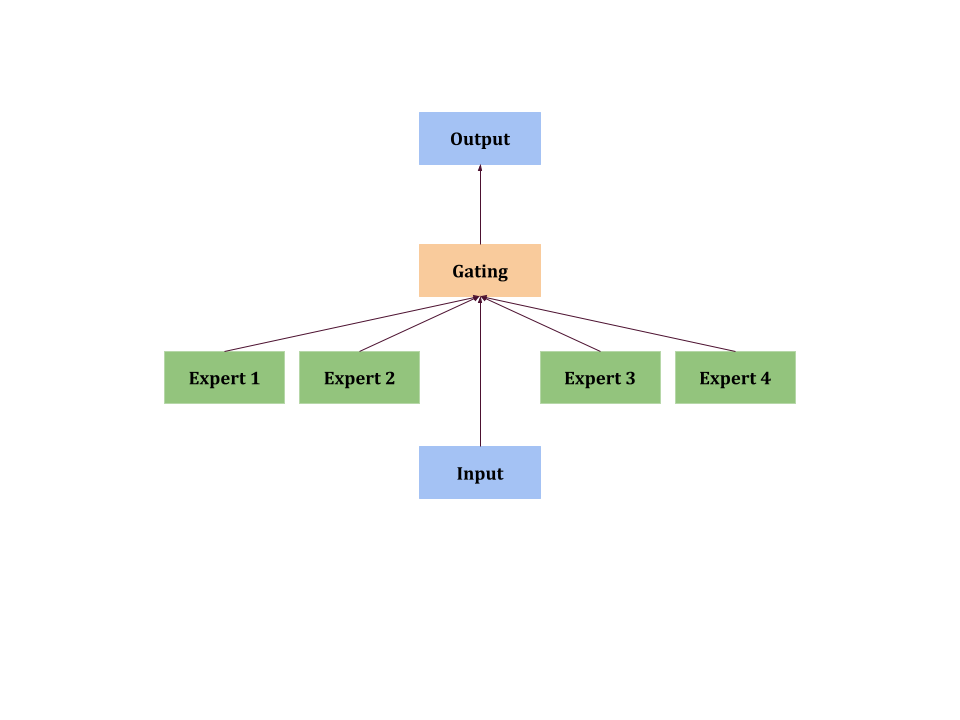
\includegraphics[width=12cm]{images/MoE.png}
    \centering
\end{figure}

\begin{figure}[ht]
    \caption{A broad overview of the proposed architecture. The unsupervised portion uses the information gained from the RLHF portion and MixCL to train the individual experts, then returned to the RLHF portion in a cycle. An initial CoT sample set is passed to a generative model used by the RLHF portion.}
    \label{fig:moe}
    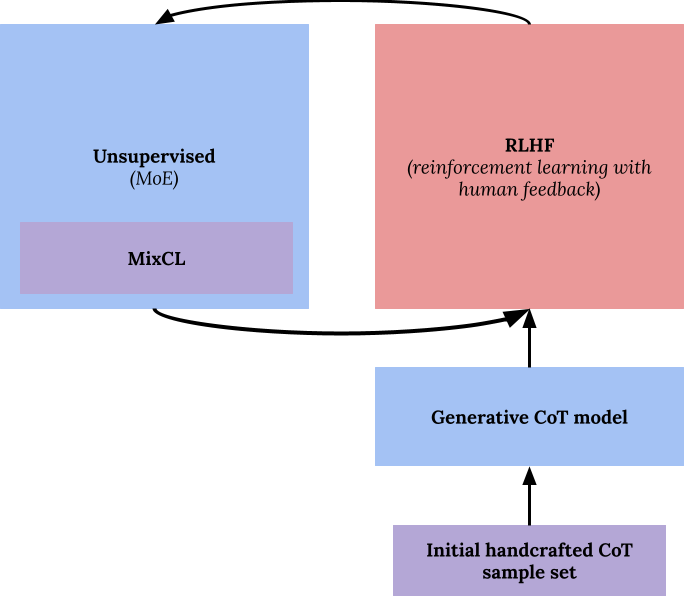
\includegraphics[width=12cm]{images/arch.png}
    \centering
\end{figure}

In order to improve the explanations of large language models, I propose the generation of a large set of appropriately explained responses using prompt engineering techniques to serve as a sample size, such as \cite{wei2022chain} \cite{scidebug}, during the reinforcement learning with human feedback (RLHF) component. At scale, it is infeasible for humans to generate a very large set, so we propose training a generative model on a small dataset of sample human-created prompts, which may then be used to expand the sample size through unsupervised learning and inference. These responses should be incorporated in the feedback loop created by the combination of RLHF and unsupervised learning. We also propose that human reviewers in the RLHF segment emphasize how well a model explains its answer to an engineered prompt in deciding whether a response to a knowledge question is ``good."

Uncertainty estimation is the final component in the proposal to improve accuracy in large language models. This should be integrated into the training cycle through a gating model, i.e. the one employed by GPT-4's Mixture-of-Experts (MoE) approach (\cref{fig:moe}). Using each of the expert models' responses as input, the gating model will perform semantic uncertainty calculations defined by Kuhn et. al. \cite{kuhn2023semantic} and improved upon by Duan et. al. \cite{duan2023shifting} and described in \cref{sec:semantic-uncertainty} to determine the ``best" response, which is then provided to the user as the output. This, while a necessary step towards improving accuracy in large language models, is insufficient without acknowledging to the user where uncertainty may exist. Therefore, we propose the addition of an external service which employs semantic uncertainty calculations on a per-sentence basis to highlight where the model may be uncertain. Alternatively, the model could provide the semantic uncertainty to the user directly.

\section{Future Work}
While \cref{sec:proposed-method} describes potential broad architectural changes based on that of GPT-3 and GPT-4, it does not explain precise implementation details, nor does it provide a proof-of-concept to demonstrate its effectiveness. Future work will entail creating and testing a working design to determine whether these architectural modifications do, in fact, lead to substantive improvements in model accuracy, explainability, and reductions in hallucinations.

Future research will also explore alternative methods for determining uncertainty in LLM responses. One such question is whether more ``human" responses are necessarily correlated with higher accuracy or ``truthfulness." If there is such a correlation, one such method for improving accuracy may involve an approach similar to that of a Generative Adversarial Network, where the LLM seeks to maximize the ``human" aspect of its responses, to make it as indistinguishable as possible from a human response.

\section{Conclusion}
This paper reviews three main issues with current state-of-the-art LLMs and approaches to improve their qualities. These are hallucinations, explainability, and uncertainty. We explore several approaches to mitigate these issues independently, such as MixCl (\cref{sec:mixcl}), CoT prompting (\cref{sec:cot}), and semantic uncertainty (\cref{sec:semantic-uncertainty}), respectively. Then, we propose a set of modifications to the structure of the GPT-series of models to integrate the MixCL, CoT prompting, and semantic uncertainty calculations together into a cohesive feedback loop which may be successful.

Advancing these qualities of LLMs together is crucial for making large language model-based approaches more viable across a wide suite of use cases. As an example, more powerful LLMs may lead to effectively providing answers in general knowledge tasks typically reserved for a search engine, greatly improving productivity, or in carrying out writing tasks without incorporating ``hallucinated," unwanted details. It is insufficient to address these problems (hallucinations, explainability, or uncertainty) independently; solutions must be integrated with each other to advance the entire state of large language models so they are more accurate, better able to reflect their level of certainty, and can explain themselves more competently. This will help LLMs become more useful tools for all aspects of society.

\printbibliography

\end{document}